% ============================================================
% Question Bank: ch03-01 Integers and Their Opposites (Modified — VA)
% Topic Title: Integers and Their Opposites (VA SOL rational number emphasis)
% CCSS: 7.NS.A.1 (Modified)
% Questions: 30 (18 MC + 7 SA + 5 Graphical)
% ============================================================

% --- Multiple Choice Questions (18) ---

\begin{practiceQuestion}{m-3-1-q01}{mc}
\begin{questionText}
What is the opposite of $-11$?
\end{questionText}
\choiceA{$-11$}
\choiceB{$0$}
\choiceC{$11$}
\choiceD{$\frac{1}{11}$}
\correctAnswer{C}
\explanation{The opposite of $-11$ is $11$ because both are $11$ units from $0$ on opposite sides.}
\end{practiceQuestion}

\begin{practiceQuestion}{m-3-1-q02}{mc}
\begin{questionText}
Which inequality correctly compares $-\dfrac{2}{3}$ and $-0.5$?
\end{questionText}
\choiceA{$-\dfrac{2}{3} > -0.5$}
\choiceB{$-\dfrac{2}{3} < -0.5$}
\choiceC{$-\dfrac{2}{3} = -0.5$}
\choiceD{Cannot be compared}
\correctAnswer{B}
\explanation{$-\frac{2}{3} \approx -0.667$. Since $-0.667 < -0.5$ (farther left on the number line), $-\frac{2}{3} < -0.5$.}
\end{practiceQuestion}

\begin{practiceQuestion}{m-3-1-q03}{mc}
\begin{questionText}
Which list is ordered from least to greatest?
\end{questionText}
\choiceA{$-1, \; -0.75, \; -\frac{1}{4}, \; 0.3, \; \frac{1}{2}$}
\choiceB{$\frac{1}{2}, \; 0.3, \; -\frac{1}{4}, \; -0.75, \; -1$}
\choiceC{$-0.75, \; -1, \; -\frac{1}{4}, \; \frac{1}{2}, \; 0.3$}
\choiceD{$-\frac{1}{4}, \; -0.75, \; -1, \; 0.3, \; \frac{1}{2}$}
\correctAnswer{A}
\explanation{Convert: $-1, -0.75, -0.25, 0.3, 0.5$. From most negative to most positive: A is correct.}
\end{practiceQuestion}

\begin{practiceQuestion}{m-3-1-q04}{mc}
\begin{questionText}
What is $|{-15}|$?
\end{questionText}
\choiceA{$-15$}
\choiceB{$15$}
\choiceC{$0$}
\choiceD{$\frac{1}{15}$}
\correctAnswer{B}
\explanation{Absolute value is distance from $0$, which is always $\geq 0$. $|{-15}| = 15$.}
\end{practiceQuestion}

\begin{practiceQuestion}{m-3-1-q05}{mc}
\begin{questionText}
Which is true: $|-3|$ \rule{0.5cm}{0.4pt} $|2|$?
\end{questionText}
\choiceA{$|-3| < |2|$}
\choiceB{$|-3| = |2|$}
\choiceC{$|-3| > |2|$}
\choiceD{Cannot be determined}
\correctAnswer{C}
\explanation{$|-3| = 3$ and $|2| = 2$. Since $3 > 2$, $|-3| > |2|$.}
\end{practiceQuestion}

\begin{practiceQuestion}{m-3-1-q06}{mc}
\begin{questionText}
Order from least to greatest: $-1.5, \; \dfrac{3}{4}, \; -\dfrac{7}{4}, \; 0.2, \; -1$.
\end{questionText}
\choiceA{$-\frac{7}{4}, \; -1.5, \; -1, \; 0.2, \; \frac{3}{4}$}
\choiceB{$-1.5, \; -\frac{7}{4}, \; -1, \; 0.2, \; \frac{3}{4}$}
\choiceC{$-1, \; -1.5, \; -\frac{7}{4}, \; 0.2, \; \frac{3}{4}$}
\choiceD{$\frac{3}{4}, \; 0.2, \; -1, \; -1.5, \; -\frac{7}{4}$}
\correctAnswer{A}
\explanation{Convert: $-1.5, 0.75, -1.75, 0.2, -1$. Order: $-1.75 < -1.5 < -1 < 0.2 < 0.75$.}
\end{practiceQuestion}

\begin{practiceQuestion}{m-3-1-q07}{mc}
\begin{questionText}
Use $<$, $>$, or $=$ to compare: $-\dfrac{3}{5}$ \rule{0.5cm}{0.4pt} $-\dfrac{1}{2}$.
\end{questionText}
\choiceA{$-\frac{3}{5} > -\frac{1}{2}$}
\choiceB{$-\frac{3}{5} < -\frac{1}{2}$}
\choiceC{$-\frac{3}{5} = -\frac{1}{2}$}
\choiceD{Cannot be determined}
\correctAnswer{B}
\explanation{$-\frac{3}{5} = -0.6$ and $-\frac{1}{2} = -0.5$. Since $-0.6 < -0.5$, $-\frac{3}{5} < -\frac{1}{2}$.}
\end{practiceQuestion}

\begin{practiceQuestion}{m-3-1-q08}{mc}
\begin{questionText}
A number plus its opposite always equals:
\end{questionText}
\choiceA{$1$}
\choiceB{$-1$}
\choiceC{$0$}
\choiceD{The number itself}
\correctAnswer{C}
\explanation{Additive inverses sum to $0$: $n + (-n) = 0$.}
\end{practiceQuestion}

\begin{practiceQuestion}{m-3-1-q09}{mc}
\begin{questionText}
Which integer is its own opposite?
\end{questionText}
\choiceA{$1$}
\choiceB{$-1$}
\choiceC{$0$}
\choiceD{No integer is its own opposite}
\correctAnswer{C}
\explanation{$0 + 0 = 0$. Zero is the only number equal to its own opposite.}
\end{practiceQuestion}

\begin{practiceQuestion}{m-3-1-q10}{mc}
\begin{questionText}
Which shows the numbers in order from greatest to least?
\end{questionText}
\choiceA{$0.4, \; -0.6, \; \frac{1}{3}, \; -\frac{3}{4}$}
\choiceB{$0.4, \; \frac{1}{3}, \; -0.6, \; -\frac{3}{4}$}
\choiceC{$-\frac{3}{4}, \; -0.6, \; \frac{1}{3}, \; 0.4$}
\choiceD{$\frac{1}{3}, \; 0.4, \; -0.6, \; -\frac{3}{4}$}
\correctAnswer{B}
\explanation{Convert: $0.4, 0.333, -0.6, -0.75$. Greatest to least: $0.4 > 0.333 > -0.6 > -0.75$.}
\end{practiceQuestion}

\begin{practiceQuestion}{m-3-1-q11}{mc}
\begin{questionText}
On a number line, which point is farther from $0$: $-4.5$ or $3.8$?
\end{questionText}
\choiceA{$3.8$}
\choiceB{$-4.5$}
\choiceC{They are equal distance}
\choiceD{Cannot be determined}
\correctAnswer{B}
\explanation{$|-4.5| = 4.5$ and $|3.8| = 3.8$. Since $4.5 > 3.8$, $-4.5$ is farther from $0$.}
\end{practiceQuestion}

\begin{practiceQuestion}{m-3-1-q12}{mc}
\begin{questionText}
Which inequality is TRUE?
\end{questionText}
\choiceA{$-\frac{5}{8} > -\frac{3}{8}$}
\choiceB{$\frac{2}{5} < -\frac{3}{5}$}
\choiceC{$-0.9 < -0.3$}
\choiceD{$-2 > -1$}
\correctAnswer{C}
\explanation{$-0.9$ is farther left on the number line than $-0.3$, so $-0.9 < -0.3$.}
\end{practiceQuestion}

\begin{practiceQuestion}{m-3-1-q13}{mc}
\begin{questionText}
Convert $-\dfrac{5}{8}$ to a decimal and compare it with $-0.6$. Which is correct?
\end{questionText}
\choiceA{$-\frac{5}{8} > -0.6$}
\choiceB{$-\frac{5}{8} < -0.6$}
\choiceC{$-\frac{5}{8} = -0.6$}
\choiceD{Cannot be determined}
\correctAnswer{B}
\explanation{$-\frac{5}{8} = -0.625$. Since $-0.625 < -0.6$, $-\frac{5}{8}$ is less.}
\end{practiceQuestion}

\begin{practiceQuestion}{m-3-1-q14}{mc}
\begin{questionText}
The temperature is $-3.5°$C. It rises $3.5°$C. What is the new temperature?
\end{questionText}
\choiceA{$-7°$C}
\choiceB{$7°$C}
\choiceC{$0°$C}
\choiceD{$3.5°$C}
\correctAnswer{C}
\explanation{$-3.5 + 3.5 = 0$. A number plus its opposite equals $0$.}
\end{practiceQuestion}

\begin{practiceQuestion}{m-3-1-q15}{mc}
\begin{questionText}
Place $-\dfrac{3}{2}$ and $-1.25$ on a number line. Which is true?
\end{questionText}
\choiceA{$-\frac{3}{2}$ is to the right of $-1.25$}
\choiceB{$-\frac{3}{2}$ is to the left of $-1.25$}
\choiceC{They are at the same point}
\choiceD{Neither can be placed on a number line}
\correctAnswer{B}
\explanation{$-\frac{3}{2} = -1.5$ and $-1.25$ is to its right because $-1.5 < -1.25$.}
\end{practiceQuestion}

\begin{practiceQuestion}{m-3-1-q16}{mc}
\begin{questionText}
Which set of numbers is in order from least to greatest?
\end{questionText}
\choiceA{$-2, \; -\frac{3}{2}, \; -0.5, \; \frac{1}{4}, \; 1.8$}
\choiceB{$-\frac{3}{2}, \; -2, \; -0.5, \; \frac{1}{4}, \; 1.8$}
\choiceC{$1.8, \; \frac{1}{4}, \; -0.5, \; -\frac{3}{2}, \; -2$}
\choiceD{$-0.5, \; -\frac{3}{2}, \; -2, \; \frac{1}{4}, \; 1.8$}
\correctAnswer{A}
\explanation{Convert: $-2, -1.5, -0.5, 0.25, 1.8$. This is already least to greatest.}
\end{practiceQuestion}

\begin{practiceQuestion}{m-3-1-q17}{mc}
\begin{questionText}
For which value of $n$ is $|n|$ the greatest?
\end{questionText}
\choiceA{$n = 4$}
\choiceB{$n = -6$}
\choiceC{$n = 5$}
\choiceD{$n = -3$}
\correctAnswer{B}
\explanation{$|4| = 4$, $|-6| = 6$, $|5| = 5$, $|-3| = 3$. The greatest absolute value is $6$.}
\end{practiceQuestion}

\begin{practiceQuestion}{m-3-1-q18}{mc}
\begin{questionText}
Which comparison uses the correct inequality symbol?
\end{questionText}
\choiceA{$\frac{2}{3} < \frac{5}{9}$}
\choiceB{$-0.4 > -0.25$}
\choiceC{$-\frac{7}{10} < -\frac{3}{5}$}
\choiceD{$1.5 < \frac{3}{4}$}
\correctAnswer{C}
\explanation{$-\frac{7}{10} = -0.7$ and $-\frac{3}{5} = -0.6$. Since $-0.7 < -0.6$, the inequality $-\frac{7}{10} < -\frac{3}{5}$ is correct.}
\end{practiceQuestion}

% --- Short Answer Questions (7) ---

\begin{practiceQuestion}{m-3-1-q19}{sa}
\begin{questionText}
What is the opposite of $\dfrac{3}{4}$?
\end{questionText}
\correctAnswer{$-\dfrac{3}{4}$}
\explanation{The opposite of $\frac{3}{4}$ is $-\frac{3}{4}$ because $\frac{3}{4} + (-\frac{3}{4}) = 0$.}
\end{practiceQuestion}

\begin{practiceQuestion}{m-3-1-q20}{sa}
\begin{questionText}
Compare using $<$, $>$, or $=$: $-\dfrac{4}{5}$ \rule{0.5cm}{0.4pt} $-0.75$.
\end{questionText}
\correctAnswer{$<$}
\explanation{$-\frac{4}{5} = -0.8$. Since $-0.8 < -0.75$, use $<$.}
\end{practiceQuestion}

\begin{practiceQuestion}{m-3-1-q21}{sa}
\begin{questionText}
Order from least to greatest: $0.6, \; -\dfrac{3}{4}, \; \dfrac{1}{3}, \; -0.5, \; 1$.
\end{questionText}
\correctAnswer{$-\dfrac{3}{4}, \; -0.5, \; \dfrac{1}{3}, \; 0.6, \; 1$}
\explanation{Convert: $0.6, -0.75, 0.333, -0.5, 1$. Order: $-0.75 < -0.5 < 0.333 < 0.6 < 1$.}
\end{practiceQuestion}

\begin{practiceQuestion}{m-3-1-q22}{sa}
\begin{questionText}
Find $|{-2.8}|$ and $|1.5|$. Which has the greater absolute value?
\end{questionText}
\correctAnswer{$|{-2.8}| = 2.8$ and $|1.5| = 1.5$. $-2.8$ has the greater absolute value.}
\explanation{$2.8 > 1.5$, so $-2.8$ is farther from $0$.}
\end{practiceQuestion}

\begin{practiceQuestion}{m-3-1-q23}{sa}
\begin{questionText}
A diver is at $-8.5$ feet. How far is the diver from sea level?
\end{questionText}
\correctAnswer{$8.5$ feet}
\explanation{Distance from sea level is $|-8.5| = 8.5$ feet.}
\end{practiceQuestion}

\begin{practiceQuestion}{m-3-1-q24}{sa}
\begin{questionText}
Place $-\dfrac{5}{6}$, $-0.8$, and $-\dfrac{7}{8}$ in order from least to greatest.
\end{questionText}
\correctAnswer{$-\dfrac{7}{8}, \; -\dfrac{5}{6}, \; -0.8$}
\explanation{Convert: $-\frac{5}{6} \approx -0.833$, $-0.8$, $-\frac{7}{8} = -0.875$. Order: $-0.875 < -0.833 < -0.8$.}
\end{practiceQuestion}

\begin{practiceQuestion}{m-3-1-q25}{sa}
\begin{questionText}
Is $-\dfrac{11}{4}$ greater than or less than $-2.5$? Explain.
\end{questionText}
\correctAnswer{$-\dfrac{11}{4} < -2.5$}
\explanation{$-\frac{11}{4} = -2.75$ and $-2.5 = -2.5$. Since $-2.75 < -2.5$, $-\frac{11}{4}$ is less than $-2.5$.}
\end{practiceQuestion}

% --- Graphical Questions (3 GMC + 2 GSA) ---

\begin{practiceQuestion}{m-3-1-q26}{gmc}
\begin{questionText}
The number line shows four points labeled with rational numbers. Which point represents $-\dfrac{3}{4}$?

\begin{center}
\begin{tikzpicture}[xscale=3]
  \draw[thick,->] (-1.6,0) -- (1.6,0);
  \foreach \x in {-1.5,-1,...,1.5} \draw (\x,0.06) -- (\x,-0.06) node[below] {\footnotesize $\x$};
  \fill[funRed] (-0.75,0) circle (2pt) node[above=6pt] {P};
  \fill[funBlue] (-0.5,0) circle (2pt) node[above=6pt] {Q};
  \fill[funGreen] (0.25,0) circle (2pt) node[above=6pt] {R};
  \fill[funOrange] (1.25,0) circle (2pt) node[above=6pt] {S};
\end{tikzpicture}
\end{center}
\end{questionText}
\choiceA{P}
\choiceB{Q}
\choiceC{R}
\choiceD{S}
\correctAnswer{A}
\explanation{$-\frac{3}{4} = -0.75$. Point P is at $-0.75$.}
\end{practiceQuestion}

\begin{practiceQuestion}{m-3-1-q27}{gmc}
\begin{questionText}
The number line shows various rational numbers. Which pair are opposites?

\begin{center}
\begin{tikzpicture}[xscale=2]
  \draw[thick,->] (-2.5,0) -- (2.5,0);
  \foreach \x in {-2,-1,0,1,2} \draw (\x,0.08) -- (\x,-0.08) node[below] {\footnotesize $\x$};
  \fill[funRed] (-1.5,0) circle (2.5pt) node[above=6pt] {A: $-1.5$};
  \fill[funBlue] (0.5,0) circle (2.5pt) node[above=6pt] {B: $0.5$};
  \fill[funGreen] (1.5,0) circle (2.5pt) node[above=6pt] {C: $1.5$};
  \fill[funOrange] (-0.5,0) circle (2.5pt) node[above=6pt] {D: $-0.5$};
\end{tikzpicture}
\end{center}
\end{questionText}
\choiceA{A and B}
\choiceB{A and C}
\choiceC{B and C}
\choiceD{A and D}
\correctAnswer{B}
\explanation{A is $-1.5$ and C is $1.5$. They are the same distance from $0$ on opposite sides — they are opposites.}
\end{practiceQuestion}

\begin{practiceQuestion}{m-3-1-q28}{gmc}
\begin{questionText}
The table shows fractions and their decimal equivalents. Which row is INCORRECT?

\begin{center}
\begin{tabular}{|c|c|c|}
\hline
\textbf{Row} & \textbf{Fraction} & \textbf{Decimal} \\
\hline
1 & $-\dfrac{3}{5}$ & $-0.6$ \\[4pt]
\hline
2 & $-\dfrac{1}{4}$ & $-0.25$ \\[4pt]
\hline
3 & $-\dfrac{2}{3}$ & $-0.66$ \\[4pt]
\hline
4 & $-\dfrac{7}{10}$ & $-0.7$ \\[4pt]
\hline
\end{tabular}
\end{center}
\end{questionText}
\choiceA{Row 1}
\choiceB{Row 2}
\choiceC{Row 3}
\choiceD{Row 4}
\correctAnswer{C}
\explanation{$-\frac{2}{3} = -0.\overline{6} = -0.666\ldots$, not exactly $-0.66$. The decimal is a repeating decimal, not a terminating one.}
\end{practiceQuestion}

\begin{practiceQuestion}{m-3-1-q29}{gsa}
\begin{questionText}
Plot these numbers on the number line and order them from least to greatest: $-1.25$, $\;\dfrac{3}{4}$, $\;-\dfrac{1}{2}$, $\;0.8$.

\begin{center}
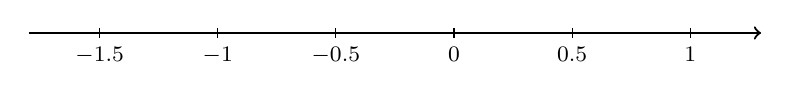
\begin{tikzpicture}[xscale=3]
  \draw[thick,->] (-1.8,0) -- (1.3,0);
  \foreach \x in {-1.5,-1,...,1} \draw (\x,0.06) -- (\x,-0.06) node[below] {\footnotesize $\x$};
\end{tikzpicture}
\end{center}
\end{questionText}
\correctAnswer{$-1.25, \; -\dfrac{1}{2}, \; \dfrac{3}{4}, \; 0.8$}
\explanation{Convert: $-1.25, 0.75, -0.5, 0.8$. Order: $-1.25 < -0.5 < 0.75 < 0.8$.}
\end{practiceQuestion}

\begin{practiceQuestion}{m-3-1-q30}{gsa}
\begin{questionText}
A thermometer shows the temperatures at four cities.

\begin{center}
\begin{tikzpicture}
  \draw[thick,->] (0,-4.5) -- (0,4.5);
  \foreach \y in {-4,...,4} {
    \draw (-0.15,\y) -- (0.15,\y);
    \node[right=4pt] at (0,\y) {\footnotesize $\y°$C};
  }
  \fill[funBlue] (0,-3.5) circle (4pt) node[left=10pt] {\footnotesize City A: $-3.5°$};
  \fill[funRed] (0,2) circle (4pt) node[left=10pt] {\footnotesize City B: $2°$};
  \fill[funGreen] (0,-1) circle (4pt) node[left=10pt] {\footnotesize City C: $-1°$};
  \fill[funOrange] (0,0.75) circle (4pt) node[left=10pt] {\footnotesize City D: $\frac{3}{4}°$};
\end{tikzpicture}
\end{center}

Order the cities from coldest to warmest and find the temperature difference between the coldest and warmest cities.
\end{questionText}
\correctAnswer{A ($-3.5°$), C ($-1°$), D ($\frac{3}{4}°$), B ($2°$). Difference: $2 - (-3.5) = 5.5°$C.}
\explanation{Coldest to warmest: $-3.5 < -1 < 0.75 < 2$. Difference: $2 - (-3.5) = 5.5°$C.}
\end{practiceQuestion}
